\documentclass[a4paper,10pt]{article}
\usepackage{graphicx}
\usepackage{amsmath}
\usepackage{hyperref}
\usepackage{geometry}
\usepackage{natbib}
\usepackage{project}
\usepackage{tikz}
\usepackage{wrapfig}
\usepackage{subcaption}
\usetikzlibrary{positioning, shapes.geometric, arrows}

\geometry{margin=1in}

\title{Interlinked Dynamics: Exploring the Correlations between Chronic Disease Indicators and Specific Death Rates}
\author{Muhammad Ahsan Khan (23491860)}
\date{\today}

\begin{document}
	\maketitle
	
	\section{Questions}
		\begin{itemize}
			\item Are there correlations between chronic disease indicators (e.g., diabetes prevalence) and specific death rates (e.g., due to heart disease)?
			\item What were the leading causes of death each year between 2020 and 2023?
		\end{itemize}
	
	\section{Data Sources}
	\subsection{Descriptions of Data Sources}
	\begin{itemize}
		\item \textbf{Datasource 1: Monthly Provisional Counts of Deaths by Select Causes (2020--2023)}
		
		The dataset includes the total counts of deaths attributed to different causes like heart disease, diabetes, cancer and COVID-19. It provides data spanning both time-related (monthly from 2020 to 2023) and geographic coverage for the United States. \cite{dataset1}
	
	\end{itemize}

	\begin{itemize}
		\item \textbf{Datasource 2: U.S. Chronic Disease Indicators (CDI)} 
		
		The dataset includes information on chronic disease indicators highlighting prevalence rates, demographic distributions and trends over time. By providing the insights of underlying health conditions that are leading to death, this dataset helps in getting a deeper understanding about the factors contributing to deaths. \cite{dataset2}
		
	\end{itemize}
	
	\subsection{Structure and Quality of Data Sources}
	\begin{itemize}
		\item \textbf{Monthly Provisional Counts of Deaths by Select Causes}
		
		The dataset represents the monthly provisional counts of deaths characterized by cause. Each columns represents distinct types of disease associated with the deaths, while the rows display the total death counts with the corresponding dates, months, years and different causes of death (e.g., heart disease, diabetes, cancer). There are a few missing values, but most columns have no missing data. Some columns are empty, however, they are not necessary for the analysis
		\begin{figure}[ht!]
			\centering
			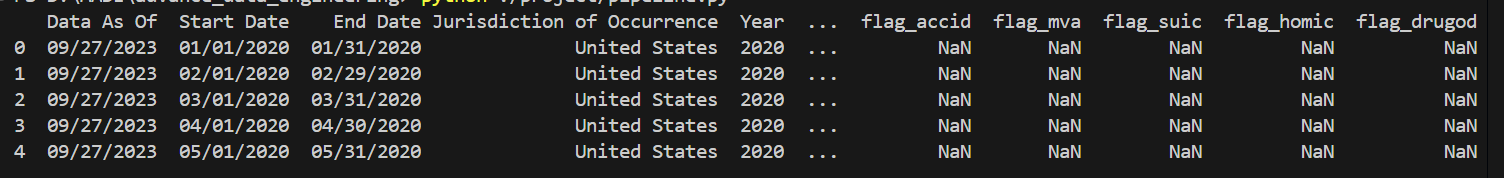
\includegraphics[width=0.9\textwidth]{images/dataset-1.png}
			\caption{First 5 rows of Monthly Provisional Counts of Deaths by Select Causes.}
			\label{fig:dataset1}
		\end{figure}
	\end{itemize}
	\begin{itemize}
		\item \textbf{U.S. Chronic Disease Indicators (CDI)} 
		
		The dataset is represented in tabular format where the rows represents health indicators and columns are grouped by demographics (e.g., gender, race, geographic location). The primary columns in the dataset are year, location, topic (indicator), questions and datavalue. Some columns are empty, however, they are not necessary for the analysis.
		\begin{figure}[ht!]
			\centering
			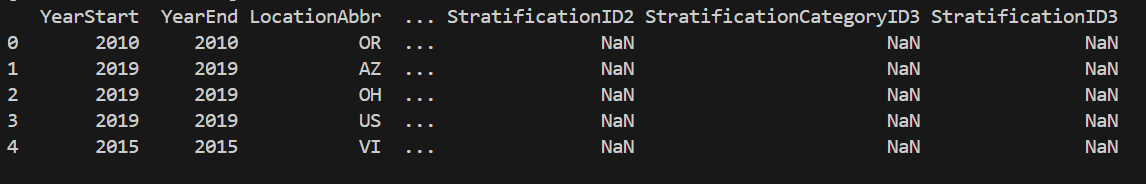
\includegraphics[width=0.9\textwidth]{images/dataset-2.png}
			\caption{First 5 rows of U.S. Chronic Disease Indicators (CDI).}
			\label{fig:dataset2}
		\end{figure}
		
	\end{itemize}

	\subsection{Licenses and Permissions}
	\begin{itemize}
	\item \textbf{Monthly Provisional Counts of Deaths by Select Causes (2020--2023)}
	
	The data is licensed under the \texttt{U.S. Government Work (Public Domain)}. The dataset is publicly available and produce by the U.S. Government. The dataset is free to use, with the only requirement being tp provide proper attribution to the U.S. government. Additionally, to ensure that no logos or other content are used in a way that implies endorsement by the U.S. government. \cite{licenses2}
	\end{itemize}
	
	\begin{itemize}
	\item \textbf{U.S. Chronic Disease Indicators (CDI)} 
		
	This dataset is available for free use under\texttt{Open Database License (ODbL)}. User are required to provide proper attribution to the original source. Additionally, any derived work must be shared under the same license. \cite{licenses1}
		
	\end{itemize}


	\subsection{Data Pipeline}
The data pipeline is developed using Python. It contains three main modules: extract, transform, load. These modules contain the following functionalities.
 
 We start by reading the metadata from a JSON file (\texttt{datasources.json}) to gather information about the data sources like URL, and columns to be removed. The process starts by extracting the data from the URL using the \texttt{CsvExtractor} function, which retrieves the dataset in a CSV. Next, unnecessary columns are removed using the \texttt{DeleteColumns} function, based on the configuration provided in the metadata. If a filtering query is specified for the dataset, the \texttt{FilterRows} function is used to filter the data accordingly. Then, empty values in the dataset are filled using the \texttt{FillEmptyValues} function to ensure completeness. Finally, the transformed dataset is loaded into the SQLite database (\texttt{ChronicHealthTrends.db}) using the \texttt{LoadDfToSqlite} function, storing the data with the appropriate dataset name.
\begin{figure}[h]
	\centering
	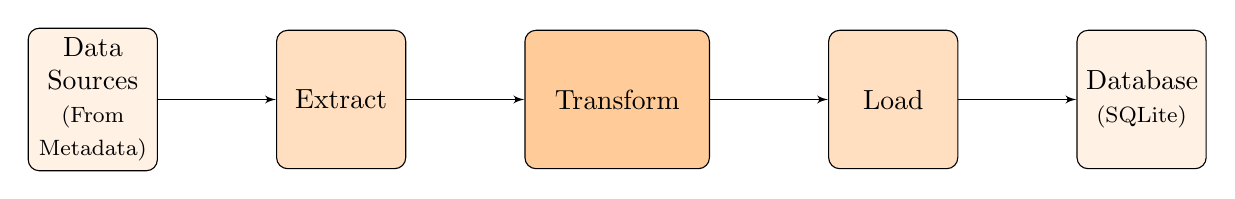
\begin{tikzpicture}[node distance=1.5cm and 1.5cm, auto]
		% Styles
		\tikzstyle{block} = [rectangle, draw, fill=orange!10,
		text width=4em, text centered, rounded corners, minimum height=5em]
		\tikzstyle{bigblock} = [rectangle, draw, fill=orange!25,
		text width=4em, text centered, rounded corners, minimum height=5em]
		\tikzstyle{biggerblock} = [rectangle, draw, fill=orange!40,
		text width=6em, text centered, rounded corners, minimum height=5em]
		\tikzstyle{line} = [draw, -latex', shorten >=0pt, shorten <=0pt]
		
		% Nodes
		\node [block] (sources) {Data Sources \footnotesize(From Metadata)};
		\node [bigblock, right=of sources] (extract) {Extract};
		\node [biggerblock, right=of extract] (transform) {Transform};
		\node [bigblock, right=of transform] (load) {Load};
		\node [block, right=of load] (database) {Database \footnotesize(SQLite)};
		
		% Connections
		\path [line] (sources) -- (extract);
		\path [line] (extract) -- (transform);
		\path [line] (transform) -- (load);
		\path [line] (load) -- (database);
	\end{tikzpicture}
	\caption{ETL Process Diagram}
	\label{fig:etl_process_diagram}
\end{figure}

	
\subsection{Results and Limitations}
The resulting datesets are stored in SQLLite in tabular format as it is the most efficient and reliable way to store collective data. The pipeline can maintain the quality of data. The resultant datasets
\begin{itemize}
	\item fulfill the requirement that is needed to answer the questions.
	\item time domain is overlapping and fitting
	\item ensure format is consistent
\end{itemize}

The datasets on chronic disease indicators and mortality statistics can be compared and analyzed to uncover correlations between chronic health conditions and mortality trends across various demographic and geographic segments. This analysis provides a detailed understanding of the underlying health factors contributing to death rates. However, a limitation exists regarding the granularity of chronic disease data, as it may not provide sufficient specificity directly link certain health indicators to the cause of mortality.






\newpage
\section{Questions}

\subsection{Are there correlations between chronic disease indicators (e.g., diabetes prevalence) and specific death rates (e.g., due to heart disease)?}

\begin{wrapfigure}{r}{0.60\textwidth} % Image aligned to the right
	\centering
	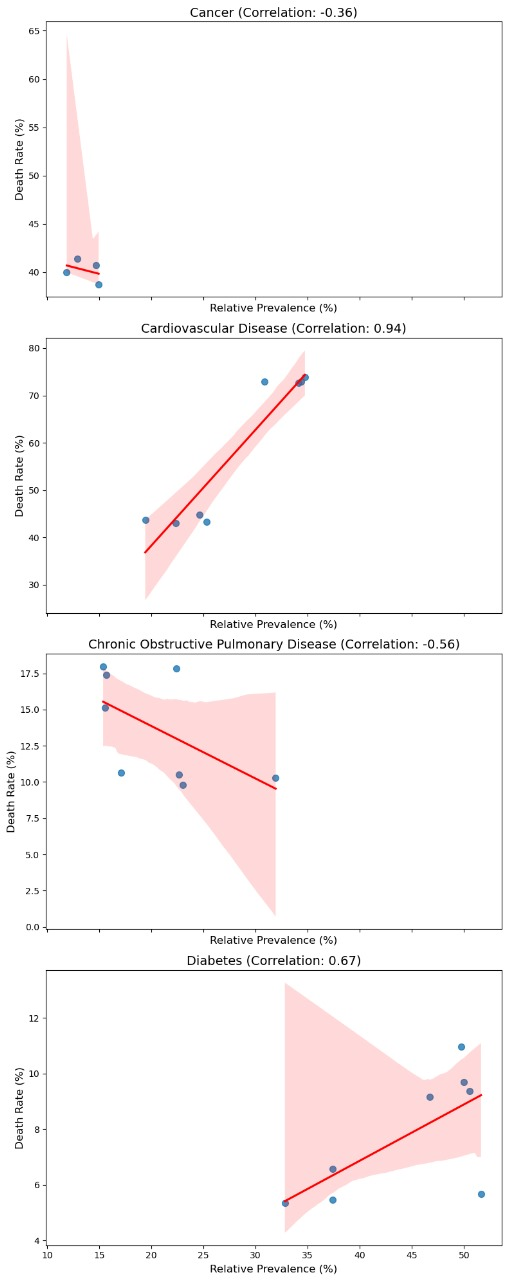
\includegraphics[width=0.38\textwidth]{images/graph-1.png} % Image file added
	\caption{Correlation Between Chronic Disease Relative Prevalence and Death Rates}
	\label{fig:scatterplot}
\end{wrapfigure}

To handle the data engineering processes, I start by building a data pipeline making sure the datasets are clean and organized for the analysis part. Initially, started by exploring the datasets individually to look for patterns or trends in the datasets. To gain more insight into the association between the chronic disease indicators and specific death rates  scatter plots with regression lines are generated. The regression lines illustrates the hidden trends and correlations. The steeper slopes signifies a stronger association. Also, the datapoints that deviated from the trend line were identified which could be assumed as potential outliers.

The outcome varied by the type of diseases as for cardiovascular diseases illustrated a strong positive correlation (of approximately 0.94), signifying a significant rise in the death rates with higher relative prevalence. Meanwhile, a moderate positive correlation was identified (of around 0.67), suggesting that the higher relative diabetes prevalence mostly coincided with higher death rates.  Contrarily, cancer illustrated a weak negative correlation (of about -0.36), indicating that the death rates are not so closely associated with the relative prevalence rate. For the Chronic Obstructive Pulmonary Disease (COPD) implied a moderate negative correlation (of about -0.56), indicating some variability in the relationship between them. The correlation for mental health was observed to be weaker, reflecting that some other factors beyond relative prevalence may have an influence over the related death rates.

\subsection{What were the leading causes of death each year between 2020 and 2023?}

To analyze the leading causes of death between the year 2020 and 2023, the dataset was filtered to extract values that lied in the range. For extracting the values, "datetime" column was incorporated aiding in comparison with the integer values that represented each year. All the irrelevant columns were excluded from the dataset including "Month", "All Cause", and "Natural Cause", only the columns related to the specific causes of deaths were kept. The death count for each disease were grouped yearly, to ensure the data was numeric and all the missing and erroneous values were handled accordingly. To identify the most prevalent diseases, only the top 5 leading causes of death based on the total death counts for each year were considered. Later, a bar plot was generated to illustrate the outcome, aggregating the causes by year and using a color scheme to differentiate among the different diseases.

\begin{figure}[ht!]
	\centering
	\begin{subfigure}[t]{0.48\textwidth}
		\centering
		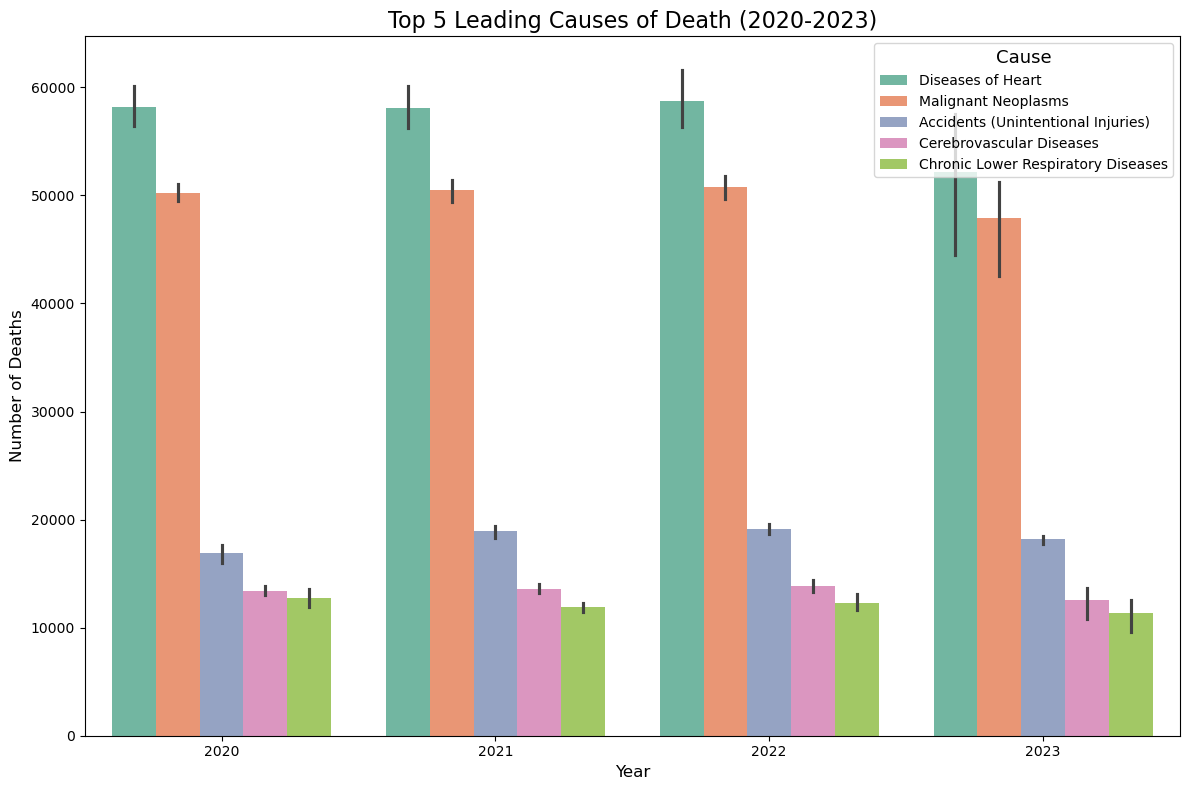
\includegraphics[width=\textwidth]{images/graph-2.png} % Image file added
		\label{fig:comparison-bar}
	\end{subfigure}
	\hfill
	\begin{subfigure}[t]{0.48\textwidth}
		\centering
		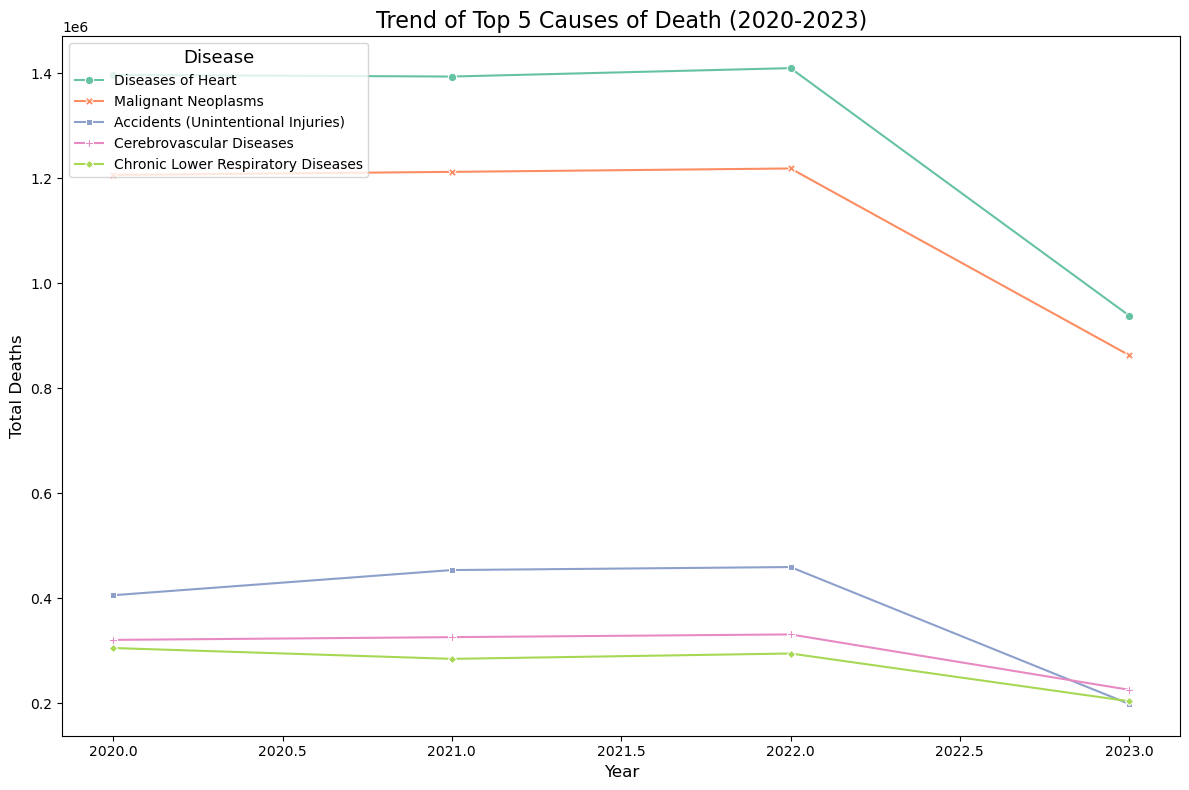
\includegraphics[width=\textwidth]{images/graph-3.png} % Image file added
		\label{fig:comparison-trend}
	\end{subfigure}
	\caption{Comparison of Top Causes of Death and Their Trends (2020-2023)}
\end{figure}

The results illustrated in the bar plot, signifies the top 5 leading causes of death from the period of 2020 to 2023. Year-over-year variation of the most significant diseases with some remaining consistent throughout the period such as the chronic diseases like cardiovascular diseases and cancer, while others varying over the duration can be observed.

\section{Conclusion}

There are links between certain death rates and indicators of chronic diseases although the strength of these associations varies per condition. While cancer and mental health have weaker association with the death rates, conditions like diabetes and cardiovascular diseases have a large positive correlation with the death rates. Furthermore, the examination of the leading causes of deaths from 2020 to 2023 indicated that, although chronic conditions continued to rank among the primary causes of death, year-to-year variations may have been impacted by outside variables or other causes.

\vspace{1em}

Although the deeper dive into the datasets highlighted the associations among the death rates and disease prevalence, this research does not support the idea of causality. It can be difficult to conclude the precise role of the chronic diseases alone because of the potential influence of outside factors on the trends illustrated. Moreover, demographics, lifestyle, and healthcare quality may all have an independent role on the death rates.

\vspace{1em}

Following are the limitations:
\begin{itemize}
	\item The analysis assumes linear relationships, which may not fully capture more complex patterns or interactions between variables.
	\item The dataset only considers shared years between datasets, which may exclude relevant trends over longer periods.
	\item Outliers and noise in the data were not deeply analyzed, potentially affecting the robustness of the results.
	\item The focus was on the top causes of death, which might overlook important secondary contributors.
\end{itemize}






\bibliographystyle{plain}
\bibliography{references}

\end{document}
